% !TeX root = ./00.ppgcc-2020.tex

\section{Article}

\subsection{Introduction}

The Internet of Things (\iot) brings together a wide variety of devices,
including mobile, wearable, consumer electronics, automotive and sensors of
various types.
% 
Such devices can either be accessed by users through the Internet or connect
to other devices, servers and applications,
with little human intervention or supervision
\cite{Tahsien2020,abane2019,haddadpajouh2019survey,Shanbhag2015}.
% 
Security and privacy is a major concern in the \iot, especially regarding
devices having access to user personal data like
location, health and many other sensitive data \cite{sengupta2020comprehensive}.
% 
Furthermore, if compromised, such devices can also be used to attack other
devices and systems, steal information, cause immediate physical damage or
perform various other malicious acts \cite{Kolias2017mirai}.
% 
As an additional concern, \iot devices likely have a long lifespan, less frequent
software patches, growing diversity of technologies combined with lack of
control over the software and hardware of such devices by the host organization
(where they are deployed), which considerably increases the attack surface.

Because most \iot devices have limited resources (i.e., battery, processing,
memory and bandwidth), configurable and expensive algorithm-based
security techniques are not usual, giving way to network based approaches 
\cite{Zhou2017}.
Machine Learning (ML) techniques, for instance, have been studied for years to detect attacks
from known patterns or to discover new attacks at an early stage
\cite{buczak2016survey,mitchell2014survey}.
A recent survey \cite{Tahsien2020} shows that ML based methods are a
promising alternative which can provide potential security tools for the \iot
network making them more reliable and accessible than before.

Despite the promising use of ML to secure \iot systems, studies found in the
literature \cite{buczak2016survey,mitchell2014survey,Tahsien2020} are limited to
traditional ML methods that use static models of traffic behavior.
Most existing ML solutions for network-based intrusion detection cannot maintain
their reliability over time when facing evolving attacks \cite{Viegas2019,AndreoniLopez2019}.
Unlike traditional methods, stream mining algorithms can be applied to intrusion
detection with several advantages, such as:

\begin{enumerate}[label=(\emph{\roman*})]
    \item processing traffic data with a single read;
    \item working with limited memory (allowing the implementation in small
    devices commonly employed in edge services);
    \item producing real-time response; and
    \item detecting novelty and changes in concepts already learned.
\end{enumerate}

Given the recent \cite{Viegas2019,AndreoniLopez2019,DaCosta2019a} use of Data Stream Novelty
Detection (\nd) in network data streams, this paper shows the effects of
adapting these mechanisms to edge services for use in \iot environments.
Our proposal, called \mfog, adapted the \arch
architecture \cite{Cassales2019a} using the \nd algorithm \minas
\cite{Faria2013Minas,Faria2015minas}, making it suitable to run
on a distributed system composed of small devices with limited
resources on the edge of the network.
Using our newer version of the \minas algorithm, we have experimentally evaluated 
how the distribution 
affects the capability to detect changes (novelty) in
traffic patterns and its impact on the computational efficiency.
Finally, some distribution strategies and policies for the data stream
novelty detection system are discussed.

This paper is organized as follows:
Section \ref{sec:minas} reviews the chosen \nd algorithm \minas.
A distributed extension of \minas, including its
implementation and evaluation are presented in Section \ref{sec:prop}
and in Section \ref{sec:experiments} we show how we evaluated \mfog and
the discuss results we found.
Finally, Section \ref{sec:conclusion} summarizes the main findings and presents
possible future work.

\subsection{Proposal}
\label{sec:prop}

In this work, we investigate an appropriate architecture for performing \nd at
the edge, as a means of allowing small IoT devices to filter and detect undesirable
network behavior.
Our approach is based on the \arch architecture \cite{Cassales2019a} and \nd
techniques provide by the \minas algorithm \cite{Faria2015minas}.
Named \mfog, our distributed algorithm explores load balancing to enable low
profile devices at the edge of the internet to also work on the classification
and detection of unwanted traffic.

In this work, we propose and assess \mfog, a distributed data stream
novelty detection system based on the algorithm \minas for securing \iot networks.
\mfog implements a distributed version of \minas according to the \arch
architecture proposed in a previous work \cite{Cassales2019a}, to execute in the
edge where small devices and constrained resources may be prevalent.

However, given the distributed nature and the typical use of small computing
devices in IoT scenarios, new challenges arise:

\begin{enumerate}[label=(\emph{\roman*})]
  \item the classification phase of the algorithm must occur in parallel at
  different nodes;
  \item the novelty detection phase, which provides the model evolution, must
  also be asynchronous;
  \item the algorithm complexity (time and space) must allow it to be processed
  by modest computing devices (i.e., small memory and low processor performance).
\end{enumerate}

\nids 
monitor network traffic, and analyze the characteristics of each flow 
to identify any intrusion or misbehavior.
However, this problem requires both fast and accurate response \cite{DaCosta2019a}:
fast response is needed to have a proper reaction before harm can be cast
to the network and to cope with the traffic without imposing loss or delay
in the \nids or observed network;
accurate response is required as not to misidentify,
especially the case of false positive that leads to false alarms.
To achieve those goals, we leverage fog computing.

In common \iot scenarios, data is captured by small devices and sent to the
cloud for any compute or storage tasks, but this is not feasible in a \nids
scenario.
Fog computing infrastructure aims to offload processing from the cloud
providers by placing edge devices closer to end-users and/or data sources.

In our proposal, fog and cloud computing resources are combined to minimize
the time elapsed between a flow descriptor ingestion and intrusion alarm,
performing the classification step of \minas running multiple
classifier instances.
After the initial classification, the resulting label can be used immediately,
but if the sample is labeled as \emph{unknown}, this sample must be stored and
the novelty detection step will be triggered.

% To have a better overview of our proposal and how it integrates with existing
% \iot environments, Figure \ref{fig:mfog-phy-arch-cloud} depicts such scenario
% showing from bottom to top:
% \iot devices directly connected to a (local) gateway network;
% this gateway network could be as simple as a single Internet router 
% or be more complex by connecting to private clouds or 
% containing more devices providing fog computing capabilities;
% lastly, available over the internet, the traditional public cloud provides
% inexpensive computing and storage on demand.
% In this scenario, the further apart resources are, the more network
% resources need to be employed, and, as with any networked system, the
% higher is the latency.

% \begin{figure}[hb]
%   \centering
%   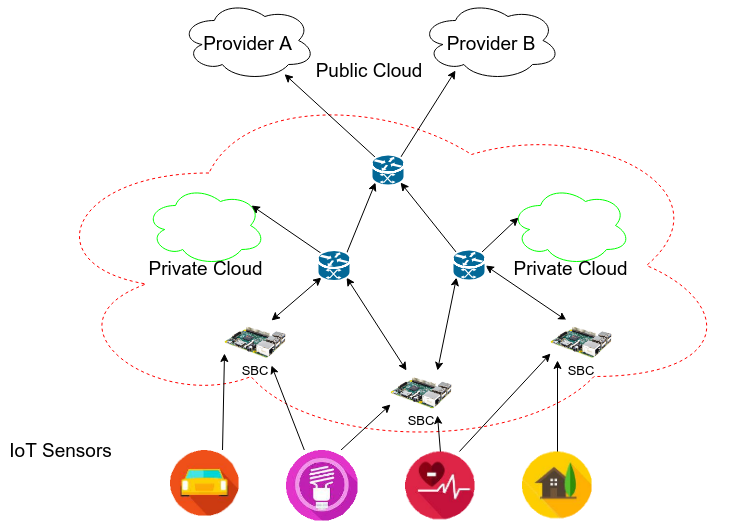
\includegraphics[width=0.5\linewidth]{figures/cassalesimgs-000.png}
%   \caption{\arch \cite{Cassales2019a} physical architecture and deployment scenario overview.}
%   \label{fig:mfog-phy-arch-cloud}
% \end{figure}

The overall \mfog architecture has two main modules, Classification and Novelty
Detection, which implement the \minas main tasks.
The Classification Module performs the same task of the \minas Online phase and
is the focal point for parallelism and distribution in our proposal.
It is replicated in the fog and runs on each cluster node, using a configurable
number of threads (limited to the node CPU core count).

The Novelty Detection Module can also be replicated,
the choice being one instance per local network, one global cloud instance,
or both.
This module also handles the homonymous task of \minas Online phase, receiving
all the samples labeled with \emph{unknown}, storing them in an internal
\emph{unknown-buffer}, and, when this buffer is full, performing the \minas
Novelty Detection task (clustering followed by validation).

\subsubsection{Polices}\label{sec:polices}

The design of our distributed \nd architecture includes partitioning the
functionalities of \minas and establishing the appropriate data flows
between different actors.
Changes to placement and behavior can have different impacts and should be
chosen with care.
The decisions following these discussions can be organized in several policies,
some of them were recurring during our implementation discussions and are:

\begin{itemize}
  \item Regarding the allocation of the Novelty Detection Module:
  \begin{itemize}
    
    \item At each fog node: patterns will be only detected if sufficient samples
    of them occur in the local observed network, use of the local node
    processing power, and a model synchronization mechanism between networks
    must be added;

    \item In the cloud: detect patterns even when scattered on each local
    network, each sample with \emph{unknown} label must be sent from edge to
    cloud implying increased internet link usage and increased delay between the
    appearance of a pattern, its detection and propagation to fog classifiers;

    \item On both: local \emph{unknown} buffer is maintained and novelty
    detection is local as well, once a sample is considered as noise or outlier
    it shall be sent to the cloud where the process repeats but with global
    data.
    This choice needs an even more complex model synchronization mechanism.

  \end{itemize}
    
  \item Regarding the model cleanup (forget mechanism): Even when a global
  novelty detection is used, local models can be optimized for faster
  classification using the local model statistics by sorting by (or removing)
  least used clusters;

  \item Lastly, reclassification of \emph{unknowns}: In the novelty detection
  task in \minas, the \emph{unknown} sample buffer is effectively classified
  using the new set of clusters.
  In Algorithm \ref{alg:MINAS-nd}, at the line \ref{alg:MINAS-nd:reclassify}, the
  new cluster valid (novelty or extension) includes the set of samples composing
  that cluster, thus, if this new label assignment was put forth to the system
  output it would introduce delayed outputs, more recent and perhaps more
  accurate.
  Also, it would change the system data stream behavior from a \emph{map}
  (meaning each input has one output) to a \emph{flatMap} (each input can have
  many outputs).

\end{itemize}


\subsubsection{Implementation}\label{sec:implementation}

The original MINAS algorithm has a companion unpublished implementation (\refminas)
written in Java using MOA library base algorithms such as K-means and CluStream,
but our implementation only used K-means.
Another difference between \refminas and \mfog is the calculus of the cluster radius 
from the distances of elements forming the cluster and the cluster's center.
\refminas uses the maximum distance while \mfog uses the standard deviation
of all distances as described in \cite{Faria2015minas}.

\newcommand{\val}{$\vec{v}\,$\xspace}
The stream formats for input and output are also of note.
As input, the algorithm takes samples (\val), which are a sequence of numbers
with dimension $d$.
In addition to \val, for both training and evaluation, the class
identifier is provided as a single character, along with a unique item identifier
(\emph{uid}), which can otherwise be determined from the sample index in the stream.

As its output, the algorithm returns the original sample \val followed by the
assigned label. Adjustments can easily be made to provide the output results as
a tuple containing \emph{uid} and the assigned label.

% - Reprocessamento dos exemplos utilizados para atualização do modelo:
%   - Muda o comportamento do operador de fluxo de `Map` para `Flatmap`, ou seja,
%     requer outro fluxo de saída para a transmissão de padrões novidade (alarmes);
%   - Para reclassificação a definição de raio é modificada de `r = f * σ` (fator
%     multiplicando desvio padrão) para `r = max(distance)` (distância máxima);
%   - Passível da crítica de *overfitting*. Isto é, este processo pode
%     inflar a métrica de precisão;
%   - **Solução:** *em aberto*;


\begin{algorithm}[htb]
% {\scriptsize
% \begin{multicols}{2}
    % \SetAlgoVlined
    \SetKwProg{Function}{Function}{:}{}
    \SetKwFor{With}{with}{}{}
    \SetKw{continue}{continue}
    % 
    \SetKwData{MEPC}{MEPC}
    \SetKwData{NF}{NF}
    \SetKwData{mpiSize}{mpiSize}
    \SetKwData{mpiRank}{mpiRank}
    \SetKwData{EndOfStream}{EndOfStream}
    % 
    \SetKwInOut{KwParams}{Parameters}
    \KwParams{mpiNodeRank as \mpiRank}
    % 
    \SetKwFunction{Mfog}{Mfog}
    \SetKwFunction{Sampler}{Sampler}
    \SetKwFunction{Classifier}{Classifier}
    \SetKwFunction{Detector}{Detector}
    \SetKwFunction{modelReceiver}{modelReceiver}
    % 
    \SetKwFunction{typeOf}{typeOf}
    % 
    \SetKwFunction{Thread}{Thread}
    \SetKwFunction{Lock}{Lock}
    \SetKwFunction{readLock}{readLock}
    \SetKwFunction{writeLock}{writeLock}
    % 
    \SetKwFunction{receive}{receive}
    \SetKwFunction{send}{send}
    \SetKwFunction{broadcast}{broadcast}
    % 
    \SetKwFunction{nearestCluster}{nearestCluster}
    \SetKwFunction{NoveltyDetection}{NoveltyDetection}
    \SetKwFunction{handleModelSleep}{handleModelSleep}
    \SetKwFunction{removeOldSamples}{removeOldSamples}
    \SetKwFunction{now}{now}
    % 
    \KwIn{ModelSet, Sample Stream}
    % \KwOut{Classified Stream as $out$}
    % 
    \Function{\Mfog{ModelStream, InputStream, OutputStream}}{
        ModelSet = $\emptyset$\;
        ModelSetLock = \textbf{new} \Lock()\;
        \eIf(\emph{root}){\mpiRank == 0}{
            \textbf{new} \Thread(\Detector, [OutputStream, ModelSet, ModelSetLock])\;
            \Sampler(InputStream, ModelSet, ModelSetLock)\;
        }(\emph{leaf}){
            \textbf{new} \Thread(\modelReceiver, [ModelSet, ModelSetLock])\;
            \Classifier(ModelSet, ModelSetLock)\;
        }
    }
\caption{MFOG: main MPI entry-point.}
\label{alg:MFOG}
\end{algorithm}

\begin{algorithm}[htb]
    \SetKwFor{With}{with}{}{}
    \SetKw{continue}{continue}
    % 
    \SetKwData{MEPC}{MEPC}
    \SetKwData{NF}{NF}
    \SetKwData{mpiSize}{mpiSize}
    \SetKwData{mpiRank}{mpiRank}
    \SetKwData{EndOfStream}{EndOfStream}
    % 
    \SetKwProg{Function}{Function}{:}{}
    \Function{\Classifier{ModelSet, ModelSetLock}}{
        \While{ True }{
            sampe = \receive(SampleType, root)\;
            \lIf{sample == \EndOfStream}{\textbf{break}}
            sample.label = unknown\;
            \With{\readLock(ModelSetLock)}{
                (distance, cluster) = \nearestCluster(sample, ModelSet)\;
            }
            \If{distance $<$ cluster.radius}{
                sample.label = cluster.label\;
            }
            \send(root, SampleType, sample)\;
        }
    }
%     \label{alg:MFOG-classifier}
%     \caption{MFOG: Classifier task.}
% \end{algorithm}
% \begin{algorithm}
    % \SetKwProg{algorithm}{algorithm}{:}{}
    \SetKwFor{With}{with}{}{}
    \SetKw{continue}{continue}
    % 
    \SetKwData{MEPC}{MEPC}
    \SetKwData{NF}{NF}
    \SetKwData{mpiSize}{mpiSize}
    \SetKwData{mpiRank}{mpiRank}
    \SetKwData{EndOfStream}{EndOfStream}
    % 
    \SetKwProg{Function}{Function}{:}{}
    \Function{\modelReceiver{ModelSet, ModelSetLock}}{
        \While{ True }{
            cl = \receive(ClusterType, root)\;
            \lIf{cl == \EndOfStream}{\textbf{break}}
            \With{writeLock(ModelSetLock)}{
                ModelSet = ModelSet $\cup$ cl\;
            }
        }
    }
    % \label{alg:MFOG-model}
    % \caption{MFOG: model receiver task.}
\caption{MFOG Leaf Tasks: Model Receiver and Classifier.}
\label{alg:MFOG-leaf}
\end{algorithm}
\begin{algorithm}[htb]
    \SetKwFor{With}{with}{}{}
    \SetKw{continue}{continue}
    % 
    \SetKwData{MEPC}{MEPC}
    \SetKwData{NF}{NF}
    \SetKwData{mpiSize}{mpiSize}
    \SetKwData{mpiRank}{mpiRank}
    \SetKwData{EndOfStream}{EndOfStream}
    \SetKwInOut{KwParams}{Parameters}
    \KwParams{mpiClusterSize as \mpiSize}
    \SetKwProg{Function}{Function}{:}{}
    \Function{\Sampler{InputStream, ModelSet, ModelSetLock}}{
        % ModelSet = read()\;
        % broadcast(ModelSet)\;
        dest = 1\;
        \ForEach{ sample from InputStream }{
            \If{\typeOf(sample) is Cluster}{
                \broadcast(ClusterType, sample, root)\;
                \With{\writeLock(ModelSetLock)}{
                    ModelSet = ModelSet $\cup$ sample\;
                }
                \continue\;
            }
            % sample.label = unknown\;
            \send(dest, SampleType, sample)\;
            dest = dest $+ 1$\;
            \lIf{dest $>$ \mpiSize}{dest = 1}
        }
    }

%     \label{alg:MFOG-sampler}
%     \caption{MFOG: sampler Module.}
% \end{algorithm}
% \begin{algorithm}
    \SetKwProg{algorithm}{algorithm}{:}{}
    \SetKwFor{With}{with}{}{}
    \SetKw{continue}{continue}
    % 
    \SetKwData{cleaningWindow}{cleaningWindow}
    \SetKwFunction{removeOldSamples}{removeOldSamples}
    \SetKwData{noveltyDetectionTrigger}{noveltyDetectionTrigger}
    \SetKwData{MEPC}{MEPC}
    \SetKwData{NF}{NF}
    \SetKwData{mpiSize}{mpiSize}
    \SetKwData{mpiRank}{mpiRank}
    \SetKwData{EndOfStream}{EndOfStream}

    \KwParams{\cleaningWindow, \noveltyDetectionTrigger}

    \SetKwProg{Function}{Function}{:}{}
    \Function{\Detector{OutputStream, ModelSet, ModelSetLock}}{
        lastCleanup $\leftarrow 0$\;
        \While{ True }{
            sampe = \receive(SampleType, any)\;
            \lIf{sample == \EndOfStream}{\textbf{break}}
            % $out \leftarrow$ sample\;
            OutputStream.append(sample)\;
            \If{sample.label == unknown}{
                UnkownSet = UnkownSet $\cup$ sample\;
                \If{$|\;UnkownSet\;| \geq$ \noveltyDetectionTrigger}{
                    novelties = \NoveltyDetection(p, ModelSet, *UnkownSet)\;
                    \With{\writeLock(ModelSetLock)}{
                        ModelSet = ModelSet $\cup$ novelties\;
                    }
                    \ForEach{ cl in novelties }{
                        \broadcast(ClusterType, cl, root)\;
                    }
                }
                \If{ sampe.uid $ > $ ( lastCleanup $ + $ \cleaningWindow )}{
                    UnkownSet $\leftarrow$ \removeOldSamples(UnkownSet, lastCleanup)\;
                    lastCleanup $ \leftarrow $ sampe.uid\;
                }
            }
        }
    }
    % \label{alg:MFOG-detector}
    % \caption{MFOG: detector task.}
\caption{MFOG Root Tasks: Sampler and Detector.}
\label{alg:MFOG-root}
\end{algorithm}

For evaluation purposes, an \mfog implementation was made using MPI (\emph{Open
MPI 4.0.4}).
The program is organized in a single program multiple data (SPMD)
programming model, so a single version of the \mfog program was initiated on all
nodes, being that one of them would perform the root role, while the others ran
as leaves, the program entry point is illustrated on Algorithm \ref{alg:MFOG}.
On the root process, a sampler thread is responsible for distributing the
sampled flow information (\val) to the classifier nodes, using a round-robin
load balancing scheme.
The other thread on the root process is responsible for receiving the
classification results and for processing the unknown samples in the search for
novelties.
The root process functions are illustrated in Algorithm \ref{alg:MFOG-root}.
Each leaf node runs a model adjustment thread and multiple (up to the number of
cores) classifier threads. The leaf tasks are illustrated in Algorithm
\ref{alg:MFOG-leaf}.
The overall sequence of interactions is shown in Figure \ref{fig:mfog-mpi-life}.

\begin{figure}[htb]
  \centerline{
    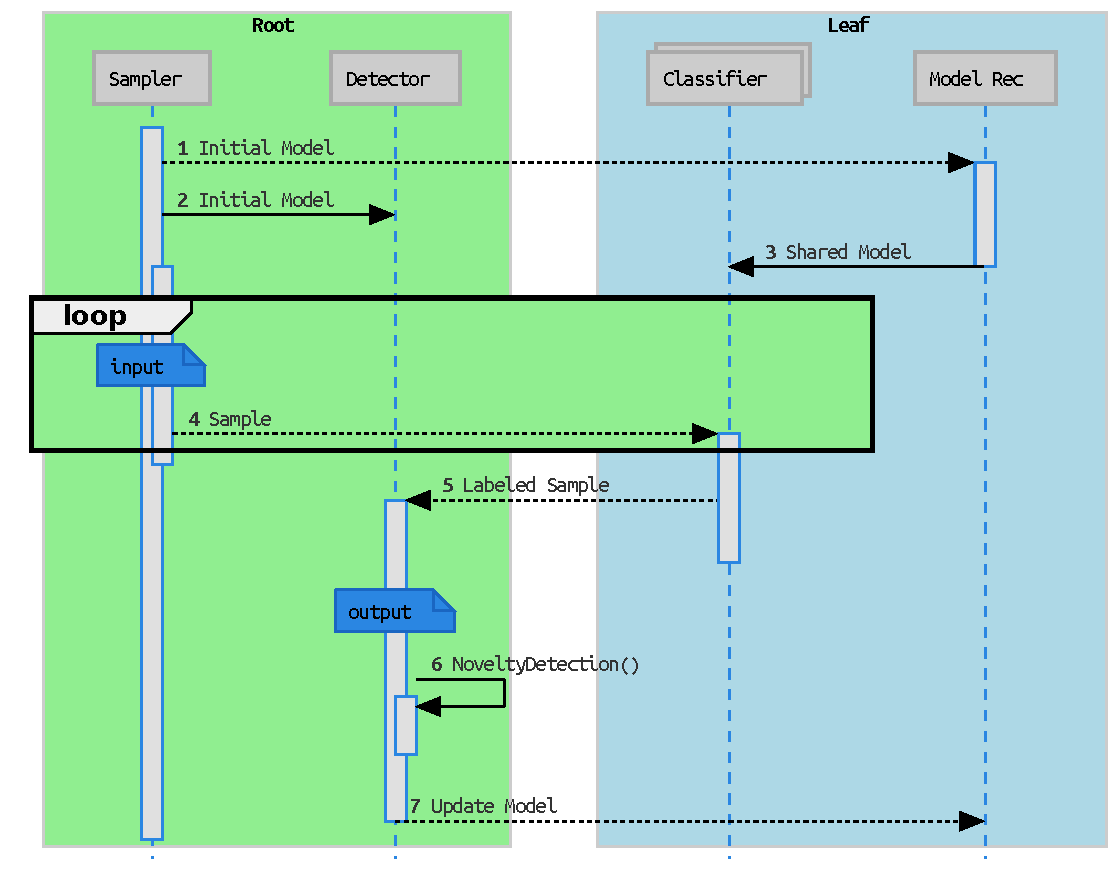
\includegraphics[width=\linewidth,page=1]{figures/lifecycle-uml-svg.pdf}
  }
  \caption{\mfog life line overview.}
  \label{fig:mfog-mpi-life}
\end{figure}


\section{Experiments and Results}
\label{sec:experiments}

% Hermes Sugestão:
% Aiming to evaluate ... what we want evaluate (ex: the distributed novelty
% detection ...) we implemented an experimental scenario composed of ... three
% dedicated Raspberry Pi 3 connected by a 100 Gbps
% Ethernet switch to simulate an IoT network with constrained resources ...
% In this scenario a trafic genenrator reproduces the network traffic of the
% data set ... describe the data set. The load generator does bla bla bla ... The

Aiming to evaluate our proposal for the effects of distributed novelty detection
in a \iot \nids scenario, we implemented an experimental setup, composed of three Raspberry Pi 3 model B single board
computers connected via Ethernet Switch. The idea was to create a simple cluster simulating an
\iot network with constrained resources at the edge of the network.
This cluster stored all source code, binaries (compiled and linked in place) and
% data sets, being accessed via our laboratory network over Secure Shell (SSH).
data sets.
In our setup, the data set is stored in the root's node SD card and is read for
each experiment.
All experiments were executed in this cluster for isolation of otherwise
unforeseen variations and for safe software comparison with constant hardware.

The data set used is the December 2015 segment of
Kyoto 2006+ data set\footnote{Available at \url{http://www.takakura.com/Kyoto\_data/}}
(Traffic Data from Kyoto University's Honeypots) \cite{Song2011}
containing $7\:865\:245$ samples.
From the original data set, we filtered only samples associated with normal traffic
or known attack types identified by existing \nids, and attack types with more
than $10\:000$ samples for significance, as previously done by
\cite{Cassales2019a}.
% , this removes 46,390 instances. TODO: revisar, pois 7M != 700K.
The remaining samples then were normalized so each feature value space (e.g., IP
Address, Duration, Service) is translated to the Real interval $[0, 1]$.

% Hermes: 72,000 em ingles usar a “,“ como separador de milhar
% SI/ISO 31-0 standard,
% Numbers consisting of long sequences of digits can be made more readable by
% separating them into groups, preferably groups of three, separated by a small
% space. For this reason, ISO 31-0 specifies that such groups of digits should
% never be separated by a comma or point, as these are reserved for use as the
% decimal sign. For example, one million (1000000) may be written as 1 000 000.

The resulting derived data set is then stored in two sets,
training set and test set, using the holdout technique.
However, for the training set we filter in only normal class
resulting in $72\:000$ instances.
For the test set we use $653\:457$ instances with
$206\:278$ instances with ``$N$'' (normal) class and
$447\:179$ instances with ``$A$'' (attack) class.
Note that this choice results in possible overfitting for the normal class and,
under-fitting for the attack class as the system first needs to detect a novel class and
then add it to the model.

% Count per class
%            id
% class        
% A      447179
% N      206278

% \begin{quote}
%   For the experiments, we used the Kyoto 2006+ data set
%   which contains data collected from 2006 to December 2015.
%   We selected examples from one month, December, 2015. Only the examples of known
%   attack types and known IDS alert code with a minimum of 10,000 occurrences (for
%   significance) were considered. The offline training was performed with 72,000
%   examples (i.e., 10\% of the data set) using the holdout technique.
%   \cite{Cassales2019a}
% \end{quote}

% \begin{highlight}
% O que quer testar com os experimentos.
% \begin{itemize}
%   \item Tese: Mostrar que detecção por novidade e classificação continua viável em fog.
%   \item Seria inviável por conta do atraso de distribuição de modelo e,
%   \item limitação pelo hardware pequeno.
%   \item MFOG: Um Agregador Regional, instalado na FOG, que observa a rede local.
% \end{itemize}

% Como realizou (cenário, rpi, setup, coleta de métricas).

% Quais resultados obteve.

% Como interpretar os resultados.
% \end{highlight}

% \hl{BEGIN Oritações de leitura das métricas e visualizações.}

\subsection{Measurements and Visualizations}

We have used two types of evaluation measurements for each experiment:
a measure of the full experiment execution time
% extracted by using \emph{GNU Time 1.9} measuring 
and, a set of qualitative measurements extracted by a Python script.

% Our script computed the
Our evaluation script was build following reference techniques like
multi-class confusion matrix with label-class association \cite{Faria2015minas}
to extract classification quality measurements.
This script takes two inputs, the test data set and the captured output stream,
and outputs the confusion matrix, label-class association,
final quality summary with:
\emph{Hits} (true positive), \emph{Misses} (Err), \emph{Unknowns} (UnkR); and
stream visualization chart with per example instance summary with novelty label markers.
% 
% For clarity, it is necessary to detail how to interpret and compare each measure,
% as for some it is trivial but others are not so much.

In the confusion matrix $M = m_{ij} \in \mathbb{N} ^{c \times{} l}$, computed by
our evaluation script, each row denotes % one of the data sets original 
the actual class $c$ and each column denotes the predicted label $l$ present in
the captured output stream.
Thus, each cell $M_{c, l}$ contains the count of examples from the test data set
of class $c$ found in the output stream with the label $l$ assigned by the under
evaluation experiment.

For the data set under use, original classes are $c \in \{N, A\}$, and for the
labels we have the training class
\emph{``N''}, \emph{unknown} label \emph{``-''} and the novelties $i \in
\mathbb{N}$ so $l \in \{N, -\} \cup \mathbb{N}$.

Added to the original confusion matrix $M$ are the rows \emph{Assigned} and
\emph{Hits}.
\emph{Assigned} row represents which original class $c$ (or if \emph{unknown},
\emph{``-''}) the label $l$ is assigned to, this is computed by using the
original class if $c = l$ or by associated novelty label to original class as
described in \cite{DeFaria2015evaluation} section 4.1
(class from where the most samples came from).
\emph{Hits} row shows the true positive count for each label $l$
with assigned class $c$, being the same value as cell $M_{c, l}$.
% computed by coping the value of the 
%  where the label is the same
% and the class $c$ is the value in the above \emph{Assigned} row.
The \emph{Hits} row is also used to compute the overall true positive
in the summary table and stream visualization chart.
% accuracy.
One complete matrix is shown in Tab. \ref{tab:java-matrix}.

% \begin{table*}[htb]
% \caption{Confusion Matrixes and Qualitative measurements}
% \label{tab:confusion-matrixes-ref-serial}

\begin{table}[hbt]%{\linewidth}
{\scriptsize
\setlength\tabcolsep{0.5em}
\begin{center}
\caption{Reference implementation}
\label{tab:java-matrix}
\begin{tabular}{l *{14}{|r} }
  Labels   &     - &       N &    1 &    2 &    3 &  4 &   5 &    6 &    7 &     8 &    9 &    10 &   11 &  12 \\\hline
  Classes  &       &         &      &      &      &    &     &      &      &       &      &       &      &     \\\hline
  \hline
  A        &  3774 &  438750 &  123 &  145 &  368 &  8 &  52 &  165 &    1 &  1046 &  161 &  2489 &   71 &  26 \\\hline
  N        &  8206 &  193030 &    0 &   79 &   44 &  0 &   0 &    0 &  229 &   181 &  154 &  4066 &  289 &   0 \\\hline
  \hline
  Assigned &     - &       N &    A &    A &    A &  A &   A &    A &    N &     A &    A &     N &    N &   A \\\hline
  Hits     &     0 &  193030 &  123 &  145 &  368 &  8 &  52 &  165 &  229 &  1046 &  161 &  4066 &  289 &  26 
\end{tabular}
\end{center}
}
\end{table}

% \vspace{3ex}

\begin{table}[hbt]%{\linewidth}
{\scriptsize
\setlength\tabcolsep{0.5em}
\begin{center}
\caption{Serial implementation}
\label{tab:libc-matrix}
\begin{tabular}{l|r|r|r|r|r|r|r|r|r|r|r}
  Labels &      - &       N &   0 &    1 &    2 &   4 &   5 &  6 &   7 &   8 &  10 \\\hline
  Classes  &        &         &     &      &      &     &     &    &     &     &     \\\hline
  \hline
  A        &  16086 &  429765 &  94 &  995 &  104 &   0 &  23 &  3 &  29 &  46 &  34 \\\hline
  N        &  12481 &  193642 &   3 &   94 &    0 &  47 &   0 &  0 &   0 &  11 &   0 \\\hline
  \hline
  Assigned &      - &       N &   A &    A &    A &   N &   A &  A &   A &   A &   A \\\hline
  Hits     &      0 &  193642 &  94 &  995 &  104 &  47 &  23 &  3 &  29 &  46 &  34 
\end{tabular}
\end{center}
}
\end{table}

\vspace{3ex}

\begin{table}[hbt]%{0.48\linewidth}
{\scriptsize
\setlength\tabcolsep{0.35em}
\begin{center}
\caption{Parallel single-node}
\label{tab:single-node-matrix}
\begin{tabular}{l|r|r|r|r|r|r|r}
  Lab. &      - &       N &    0 &    1 &   2 &  3 &  4 \\\hline
  Cla.  &        &         &      &      &     &    &    \\\hline
  \hline
  A        &  12282 &  433797 &  147 &  952 &   0 &  0 &  1 \\\hline
  N        &   3088 &  203019 &   40 &   99 &  27 &  5 &  0 \\\hline
  \hline
  Ass. &      - &       N &    A &    A &   N &  N &  A \\\hline
  Hits     &      0 &  203019 &  147 &  952 &  27 &  5 &  1 
\end{tabular}
\end{center}
}
\end{table}
% 
% \quad
% &
% 
\begin{table}[hbt]%{0.48\linewidth}
{\scriptsize
\setlength\tabcolsep{0.35em}
\begin{center}
\caption{Parallel multi-node}
\label{tab:multi-node-matrix}
\begin{tabular}{l|r|r|r|r|r|r|r}
  Lab.   &      - &       N &    0 &    1 &    2 &    3 &  4 \\\hline
  Cla.   &        &         &      &      &      &      &    \\\hline
  \hline
  A      &  12378 &  433631 &  117 &  886 &    0 &  162 &  5 \\\hline
  N      &   3121 &  202916 &   40 &   96 &  105 &    0 &  0 \\\hline
  \hline
  Ass.   &      - &       N &    A &    A &    N &    A &  A \\\hline
  Hits   &      0 &  202916 &  117 &  886 &  105 &  162 &  5 
\end{tabular}
\end{center}
}
\end{table}

% \end{table*}

For the measurements summary table, six measurements from two sources are displayed. Three
measures \emph{Hits}, \emph{Unknowns} and \emph{Misses} represented as ratio of
the captured output stream, extracted from the evaluation python program,
computed as follows:
\emph{Hits} (true positive rate) is the sum of the \emph{Hits} row in the
extended confusion matrix;
\emph{Unknowns} is the count of examples in the captured output stream marked
with the \emph{unknown} label (\emph{``-''});
\emph{Misses} is the count of all examples in the captured output stream marked
with a label distinct from the \emph{Assigned} original class and are not marked
as unknown.

Furthermore in the measurement summary table, \emph{Time}, \emph{System} and \emph{Elapsed}
 represented in seconds, are extracted from \emph{GNU Time 1.9}.
\emph{Time} is the amount of CPU seconds expended in user-mode
(indicates time used doing CPU intensive computing, e.g., math);
\emph{System} is the amount of CPU seconds expended in kernel-mode
(for our case, it indicates time doing input or output);
\emph{Elapsed} is the real-world (wall clock) elapsed time and
indicates how long the program took to complete.
The lower the times, the better.
Our four main experiments are shown in Tab. \ref{tab:exper-summary}.

Lastly, the stream visualization chart shows the summary quality measurement
(\emph{Hits}, \emph{Unknowns}, \emph{Misses})
computed for each example in the captured output stream.
This summary is computed for each example, but it uses the \emph{Assigned} row
computed previously to evaluate \emph{Hits}; the other measurements are derived as
described before.
The Horizontal axis (x, domain) plots the index of the example and the
vertical axis (y, image) shows the measurement computed until that example index on the captured
output stream.

Adding to the stream visualization chart, novelty label markers are represented
as vertical lines indicating \emph{when} in the captured output stream a new
label first appeared.
Some of the novelty label markers include the label itself ($l \in \mathbb{N}$)
for reference (showing every label would turn this feature unreadable due
to overlapping).
Figure \ref{fig:visualization} shows complete stream visualization charts.

\begin{figure}[htb]
  \centering
  \begin{minipage}{0.48\textwidth}
    \centering
    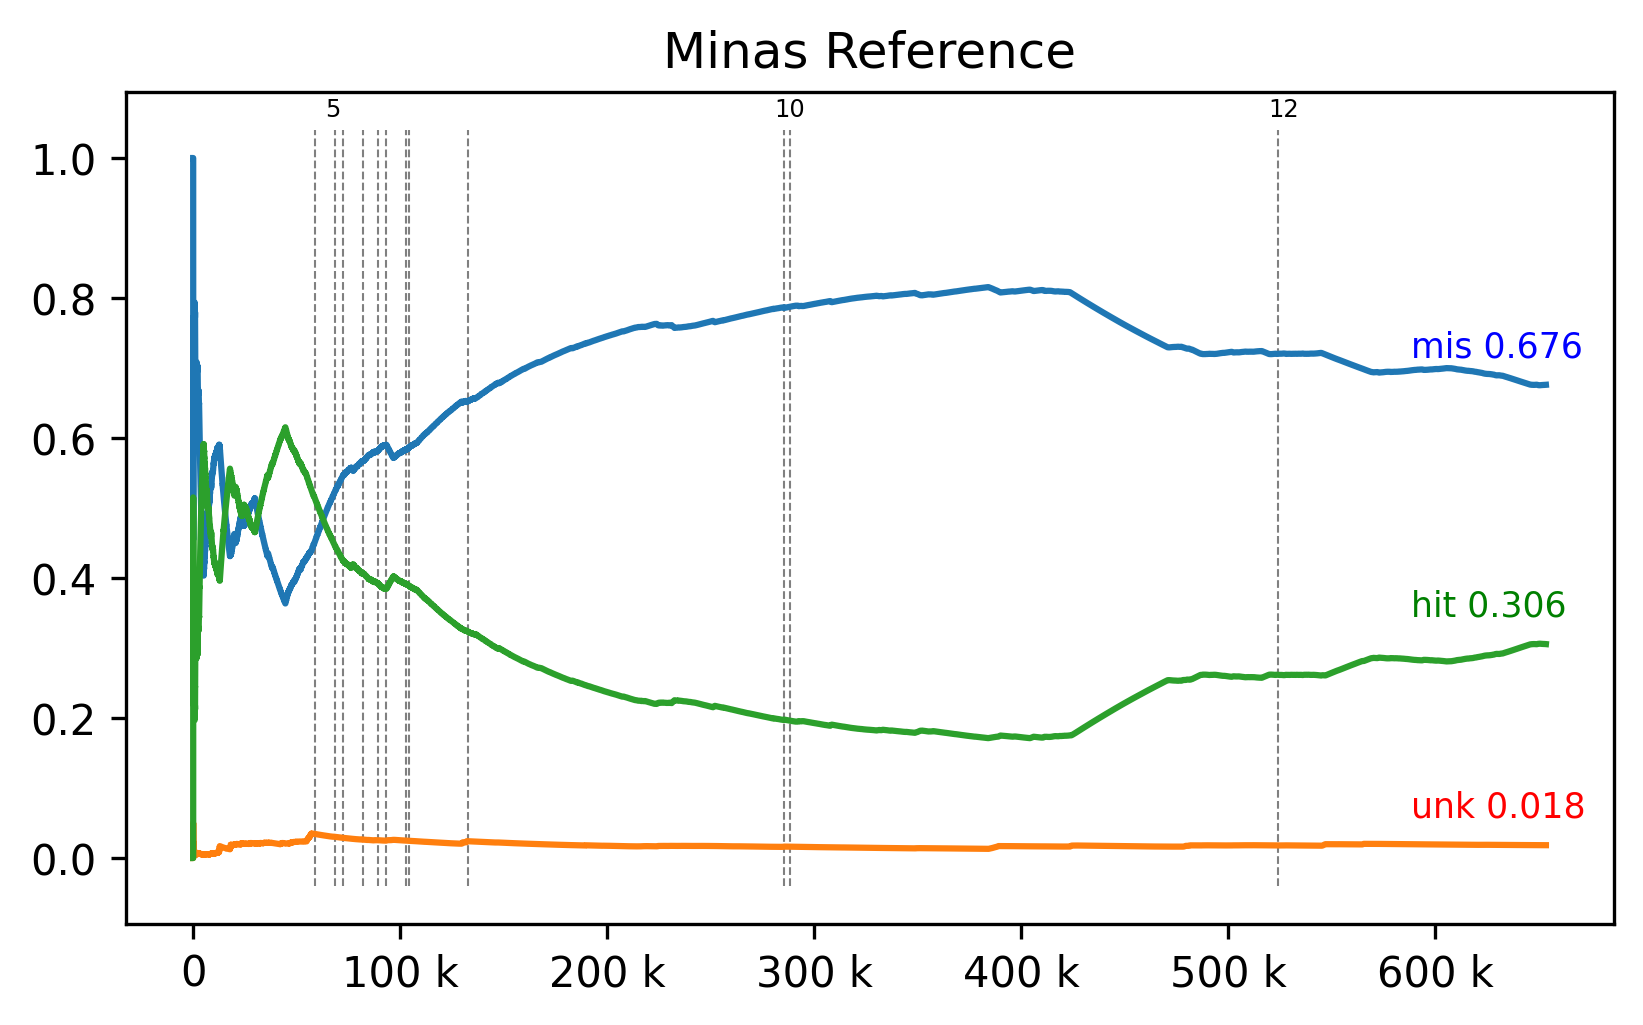
\includegraphics[width=1\linewidth]{experiments/revised-java.log.png}
    % \caption{Reference Implementation}
    \legend{Reference Implementation}
    \label{fig:validation-sub-java}
  \end{minipage}
  \hfill
  \begin{minipage}{0.48\textwidth}
    \centering
    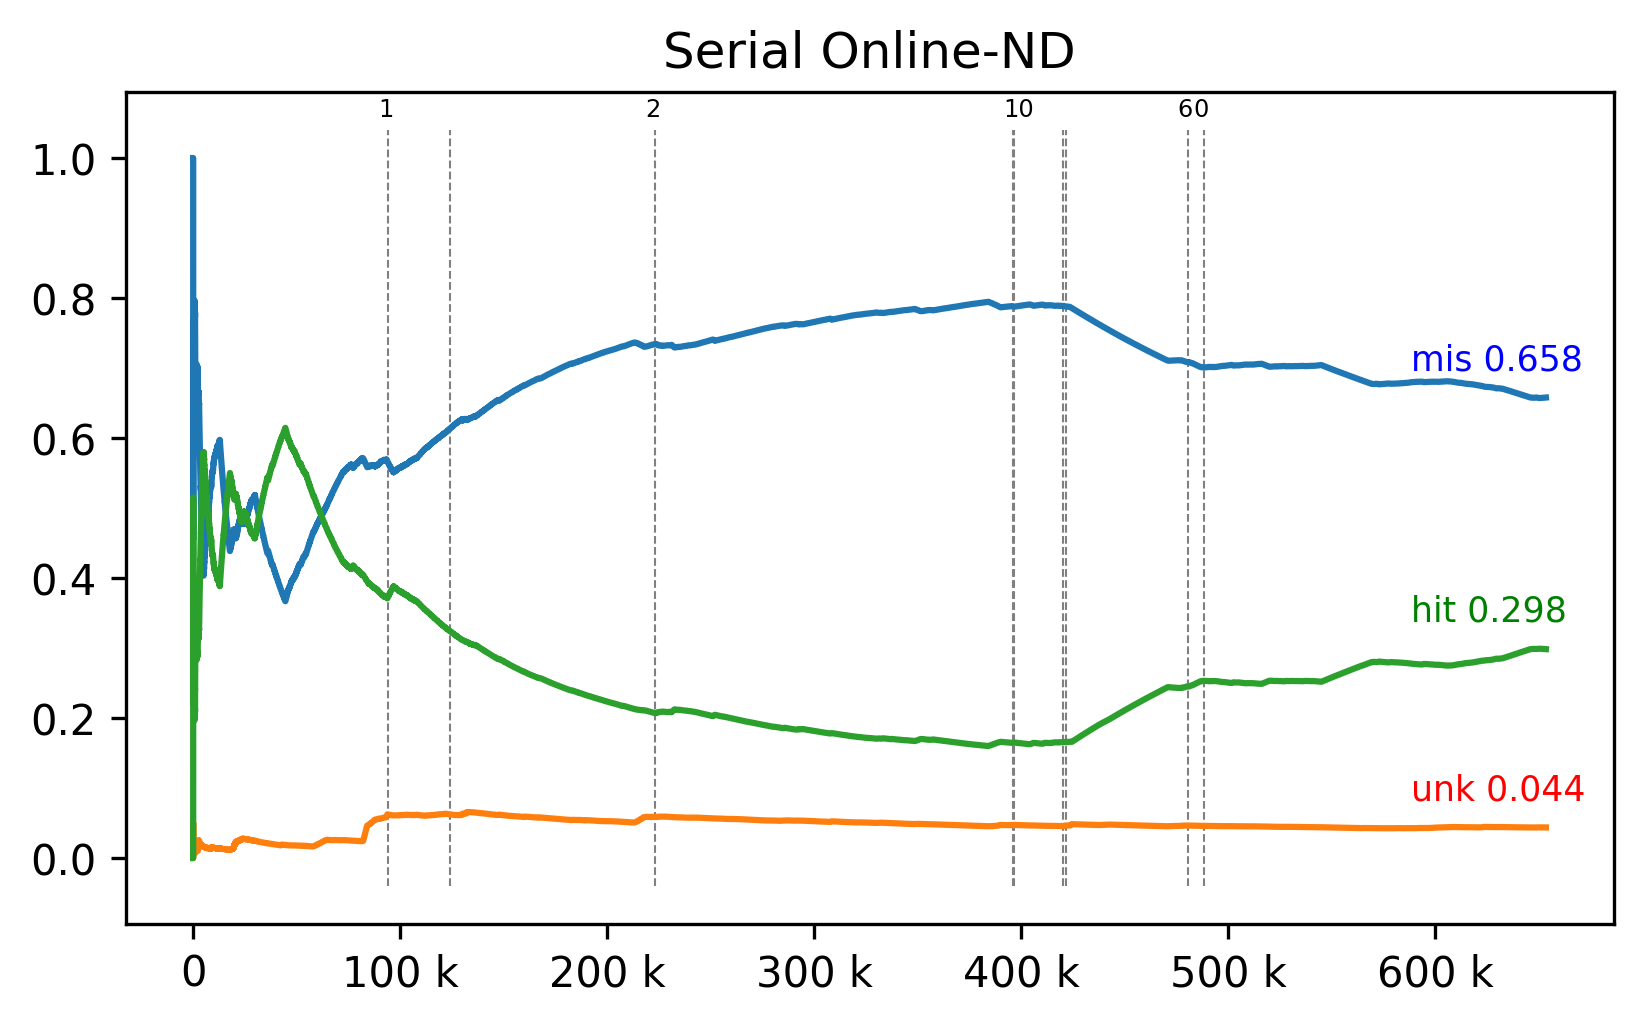
\includegraphics[width=1\linewidth]{experiments/online-nd.log.png}
    \caption{Serial Implementation}
    \label{fig:validation-sub-serial}
  \end{minipage}
  \vspace{5mm}
  \begin{minipage}{0.48\textwidth}
    \centering
    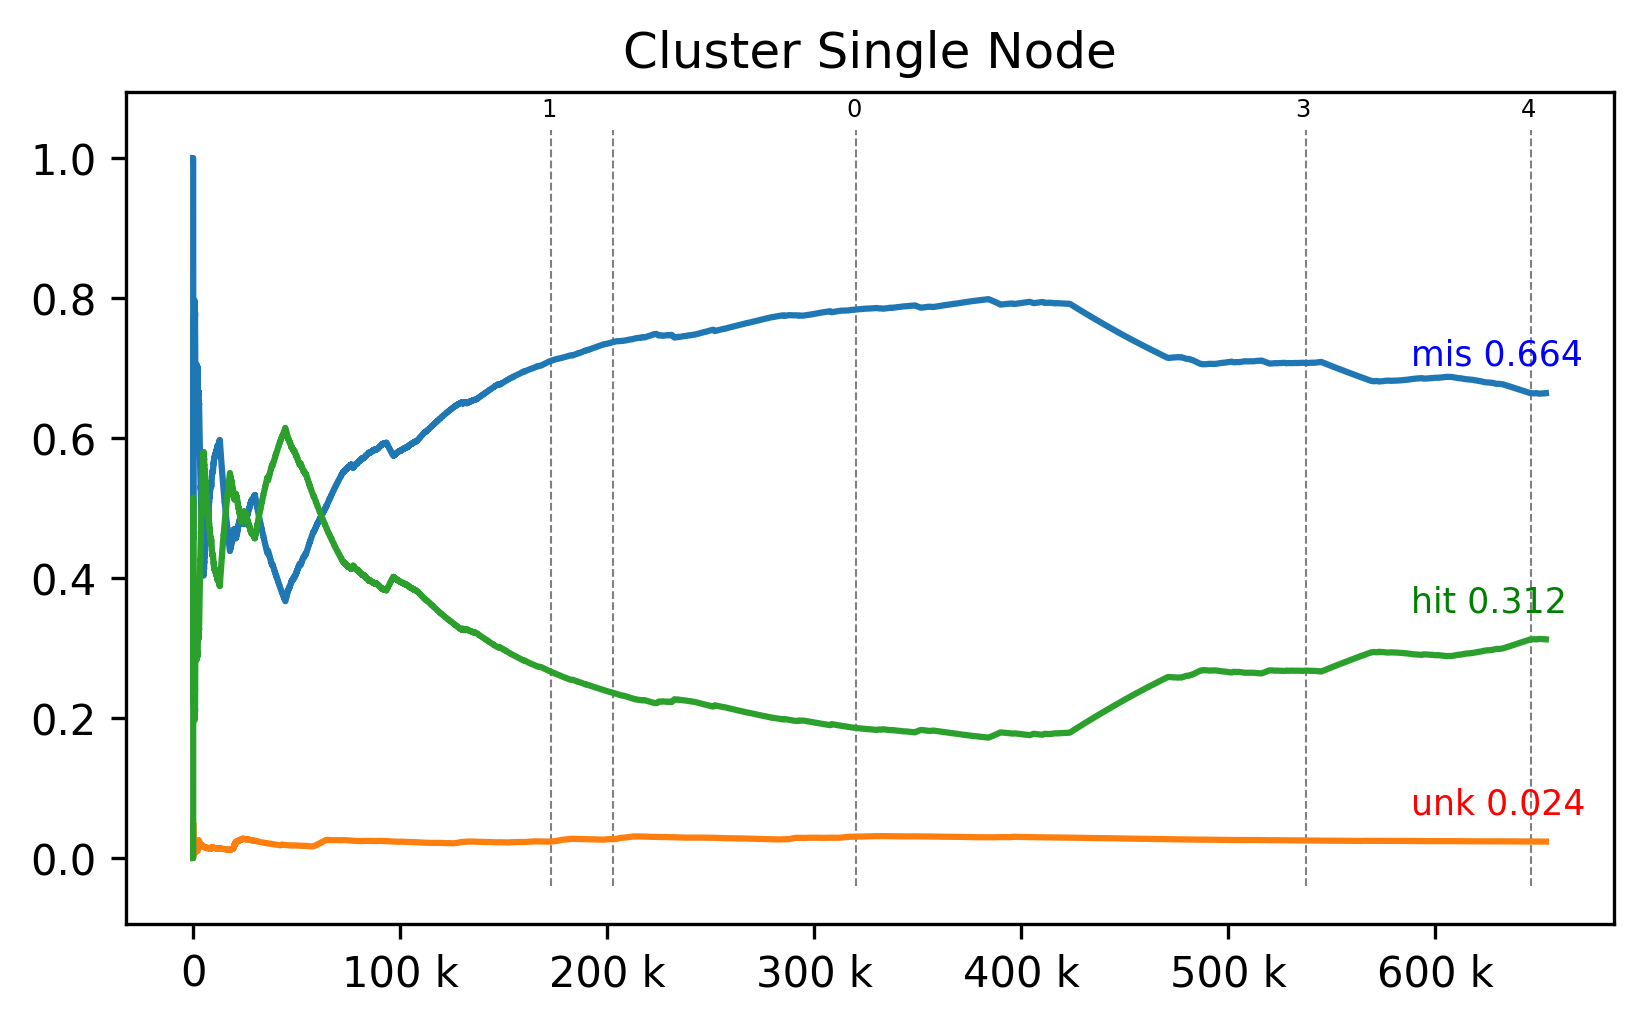
\includegraphics[width=1\linewidth]{experiments/tmi-base.log.png}
    \caption{Parallel single-node}
    \label{fig:cluster-sub-single}
  \end{minipage}
  \hfill
  \begin{minipage}{0.48\textwidth}
    \centering
    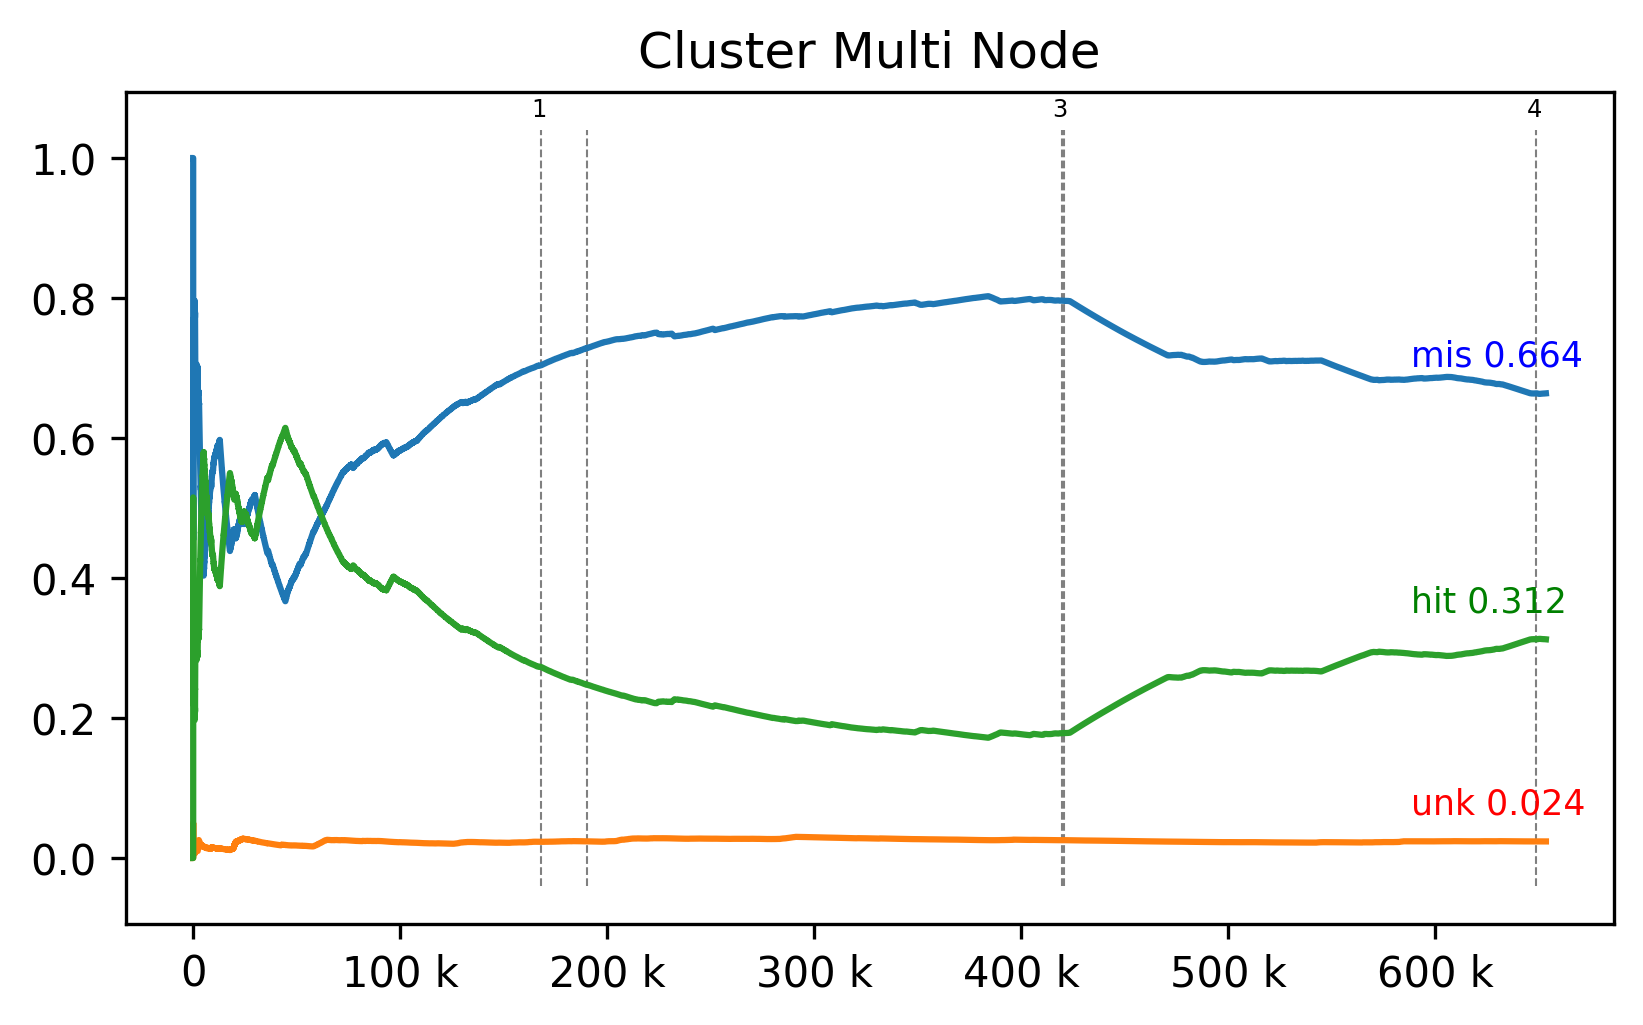
\includegraphics[width=1\linewidth]{experiments/tmi-n12.log.png}
    \caption{Parallel multi-node}
    \label{fig:cluster-sub-multi}
  \end{minipage}
  \caption{Stream hits and novelties visualization}
  \label{fig:visualization}
\end{figure}

\subsubsection{Discussion}

Four main experiments are presented for discussion:
(\emph{a}) reference implementation of Minas (\refminas) \cite{Faria2015minas};
(\emph{b}) new implementation in serial mode;
(\emph{c}) new implementation in single-node, multi-task mode and
(\emph{d}) new implementation in multi-node, multi-task mode.
Each experiment uses the adequate binary executable, initial model
(or training set for the reference implementation) and test set
to compute a resulting output stream which is stored for qualitative evaluation.
The summary of all four experiments is shown in Table \ref{tab:exper-summary}.

\begin{table*}[hbt]
\begin{center}
  \caption{Collected Measures Summary.}
  \label{tab:exper-summary}
  \newcommand{\mr}[1]{\multirow{2}{*}{#1}}
  \begin{tabular}{l|r|r|r|r|r}
                    & \refminas (a)  & Offline       & Serial (b)      & Single Node (c) & Multi Node (d)  \\\hline
    \mr{Hits}       & $\ 199708\ $   &               & $\ 195017\ $    & $\ 204151\ $    & $\ 204191\ $    \\
                    & $\ 0.305618\ $ &               & $\ 0.298438\ $  & $\ 0.312416\ $  & $\ 0.312478\ $  \\
    \hline
    \mr{Misses}     & $\ 441769\ $   &               & $\ 429873\ $    & $\ 433936\ $    & $\ 433767\ $    \\
                    & $\ 0.676049\ $ &               & $\ 0.657843\ $  & $\ 0.664061\ $  & $\ 0.663802\ $  \\
    \hline
    \mr{Unknowns}   & $\ 11980\ $    &               & $\ 28567\ $     & $\ 15370\ $     & $\ 15499\ $     \\
                    & $\ 0.018333\ $ &               & $\ 0.043717\ $  & $\ 0.023521\ $  & $\ 0.023718\ $  \\
    \hline
    Time            & $\ 2761.83\ $  & $\ 194.12\ $  & $\ 80.79000\ $  & $\ 522.1000\ $  & $\ 207.1400\ $  \\\hline
    System          & $\ 7.15\ $     & $\  0.075\ $  & $\ 11.51000\ $  & $\  47.7700\ $  & $\ 157.6100\ $  \\\hline
    Elapsed         & $\ 2772.07\ $  & $\ 194.27\ $  & $\ 93.03000\ $  & $\ 145.0400\ $  & $\  95.3800\ $  
  \end{tabular}
\end{center}
\end{table*}

The comparison of the first two experiments (\emph{a} and \emph{b}) provides a
validation for our implementation, while the latter three (\emph{b}, \emph{c}
and \emph{d}) serve as showcase for the effects of distribution.

As stated, to validate our implementation we have compared it to \refminas
(the original \minas companion implementation), so we extracted the same measurements
using same process for both \emph{a} and \emph{b}, which can be viewed in
Tables \ref{tab:java-matrix}, \ref{tab:libc-matrix} and for ease of comparison
in Table \ref{tab:exper-summary} the summary can be compared side by side.

In general, the observed classification quality measurements are very similar,
and only diverge slightly where \emph{a} has more \emph{Hits} and \emph{Misses}
whereas \emph{b} shifted those to \emph{Unknowns}.
This phenomenon was watched very closely during development and we found that it was due to
small changes to \minas parameters, \minas internals like K-means ordering,
cluster edge inclusion and cluster radius formula as stated in
Subsection \ref{sec:implementation}.

As for the time measurements in Table \ref{tab:exper-summary}
our implementation used less time to analyze the test data set.
This is mostly due to 
the stop condition
on the internal K-means algorithm; while \refminas uses a fixed iteration
limit of $100$, our implementations adds the ``no improvement'' check
and stops earlier in most cases, which in turn reduces the time taken
on the \emph{NoveltyDetection} function.
There are also small optimizations on the \emph{nearestCluster} function
(minimal distance from sample to cluster center in the set)
affecting the \emph{classifier} task and \emph{NoveltyDetection} function.
One can also note that \refminas time in \emph{a} includes the Offline phase while our
implementation runs it once and reuses the initial model for \emph{b}, \emph{c}
and \emph{d}. In the table the offline time this is shown as a separate column.

As for the effects of running the classification processes on the small devices as MPI nodes with our implementation, we observe
an increase of time when we go from $2$ to $4$ instances in a single node
(\emph{b} and \emph{c} respectively), hinting that our choice of load
distribution is not as effective as we expected.
Further experiments were conducted with the number of instances varying from $1$ (serial) to
$12$ (3 nodes with 4 CPUs each), but that caused no impact on the true positive rate (\emph{Hits}) and elapsed time.
More detailed time measurements can be seen in Figure \ref{fig:speedup},
where we observe near constant time for \emph{elapsed} (near $100s$),
the \emph{system} increases gradually while \emph{user} decreases at the same rate.
We interpret this behavior as a display of potential for gains using a better
load balancing than our choice of round-robin such as micro-batching for better
compute-to-communication ratio (CCR).
In general, Figure \ref{fig:speedup} shows no speedup but also no penalty for
scaling to more than $4$ instances.

\begin{figure}[hbt]
  \centering
  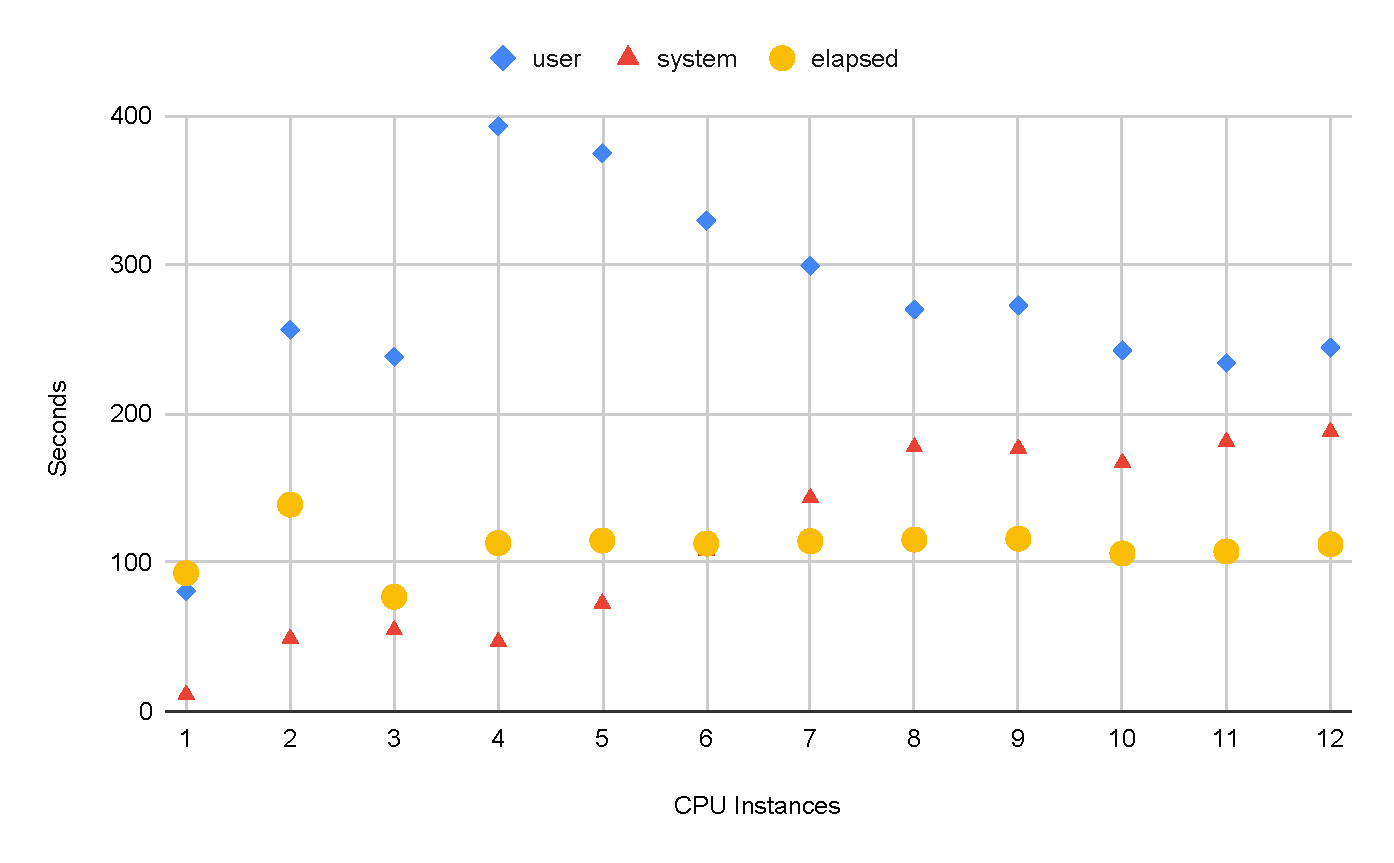
\includegraphics[width=\linewidth,page=1]{experiments/speedup-clean.pdf}
  \caption{Time measurements per added instance}
  \label{fig:speedup}
\end{figure}

Nevertheless, we can also show the effects of delay in the
Classify, Novelty Detection, Model Update and Classify feedback loop.
Comparing \emph{b} and \emph{c} we observe a reduction in Novelty labels
on the Confusion Matrix (tabs. \ref{tab:libc-matrix} and \ref{tab:single-node-matrix})
from $10$ to $4$.
The same effect is observed on the stream visualization (figs.
\ref{fig:validation-sub-serial} and \ref{fig:cluster-sub-single}) where our
serial implementation has fewer novelty markers, and they appear later, but the
measures keep the same ``shape''.
Comparing \emph{c} and \emph{d} the difference is even smaller,
(figs. \ref{fig:validation-sub-serial} and \ref{fig:cluster-sub-single})
as they both suffer the expected delay in the feedback loop.

\subsection{Conclusion}
\label{sec:conclusion}

Data Stream Novelty Detection (\nd) can be a useful mechanism for Network
Intrusion Detection (\nids) in IoT environments. It can also serve other related applications of \nd using continuous
network or system behavior monitoring and analysis.
Regarding the tremendous amount of data that must be processed in the flow analysis for \nd, it 
is relevant that this processing takes place at the edge of the network. 
However, one relevant shortcoming of the IoT, in this case, is the reduced processing capacity of such edge devices. 

In this sense, we have put together and evaluated a distributed architecture for performing \nd in network flows at the edge.
Our proposal, \mfog is a distributed \nd
implementation based on the \nd algorithm \minas.

The main goal of this work is to observe the effects of our approach to a
previously serial only algorithm, especially in regards to time and quality
metrics.

While there is some impact on the predictive metrics, this is not reflected on
overall classification quality metrics indicating that distribution of \minas
shows a negligible loss of accuracy.
In regards to time and scale, our distributed executions was faster than the 
previous sequential implementation of \minas, but efficient data distribution was not achieved as the
observed time with each added node remained constant.

Overall, \mfog and the idea of using distributed flow classification and novelty
detection while minimizing memory usage to fit in smaller devices at the edge of
the network is a viable and promising solution.
Further work include the investigation of other \nd algorithms, other clustering
algorithms in \minas and analysis of varying load balancing strategies.

\subsection*{Acknowledgment}

This study was financed in part by the Coordenação de Aperfeiçoamento de Pessoal
de Nível Superior - Brasil (CAPES) - Finance Code 001, and Programa
Institucional de Internacionalização – CAPES-PrInt UFSCar (Contract
88887.373234/2019-00). Authors also thank Stic AMSUD (project 20-STIC-09),
FAPESP (contract numbers 2018/22979-2, and 2015/24461-2) and CNPq (Contract
167345/2018-4) for their support.
